\section{Design di dettaglio}
Design di dettaglio (scelte rilevanti, pattern di progettazione, organizzazione del codice -- corredato da pochi ma efficaci diagrammi)

\subsection{Pattern di progettazione}
\subsubsection{Family polimorphism}
\subsubsection{Bounded F-polimorphism}
\subsubsection{Pimp my library}
\subsubsection{Strategy}
\subsubsection{Adapter}
\subsubsection{Factory}

\subsection{Organizzazione del codice}
Il codice è stato organizzato in packages. Questi, seguono la suddivisione in scene dell'applicativo. Al loro interno, si può ritrovare una suddivisione in Model, View, ViewModel e Componenti.
Il package Core invece, contiene le parti basilare a cui il resto del sistema fa riferimento.

\begin{figure}[!hbt]
    \centering
    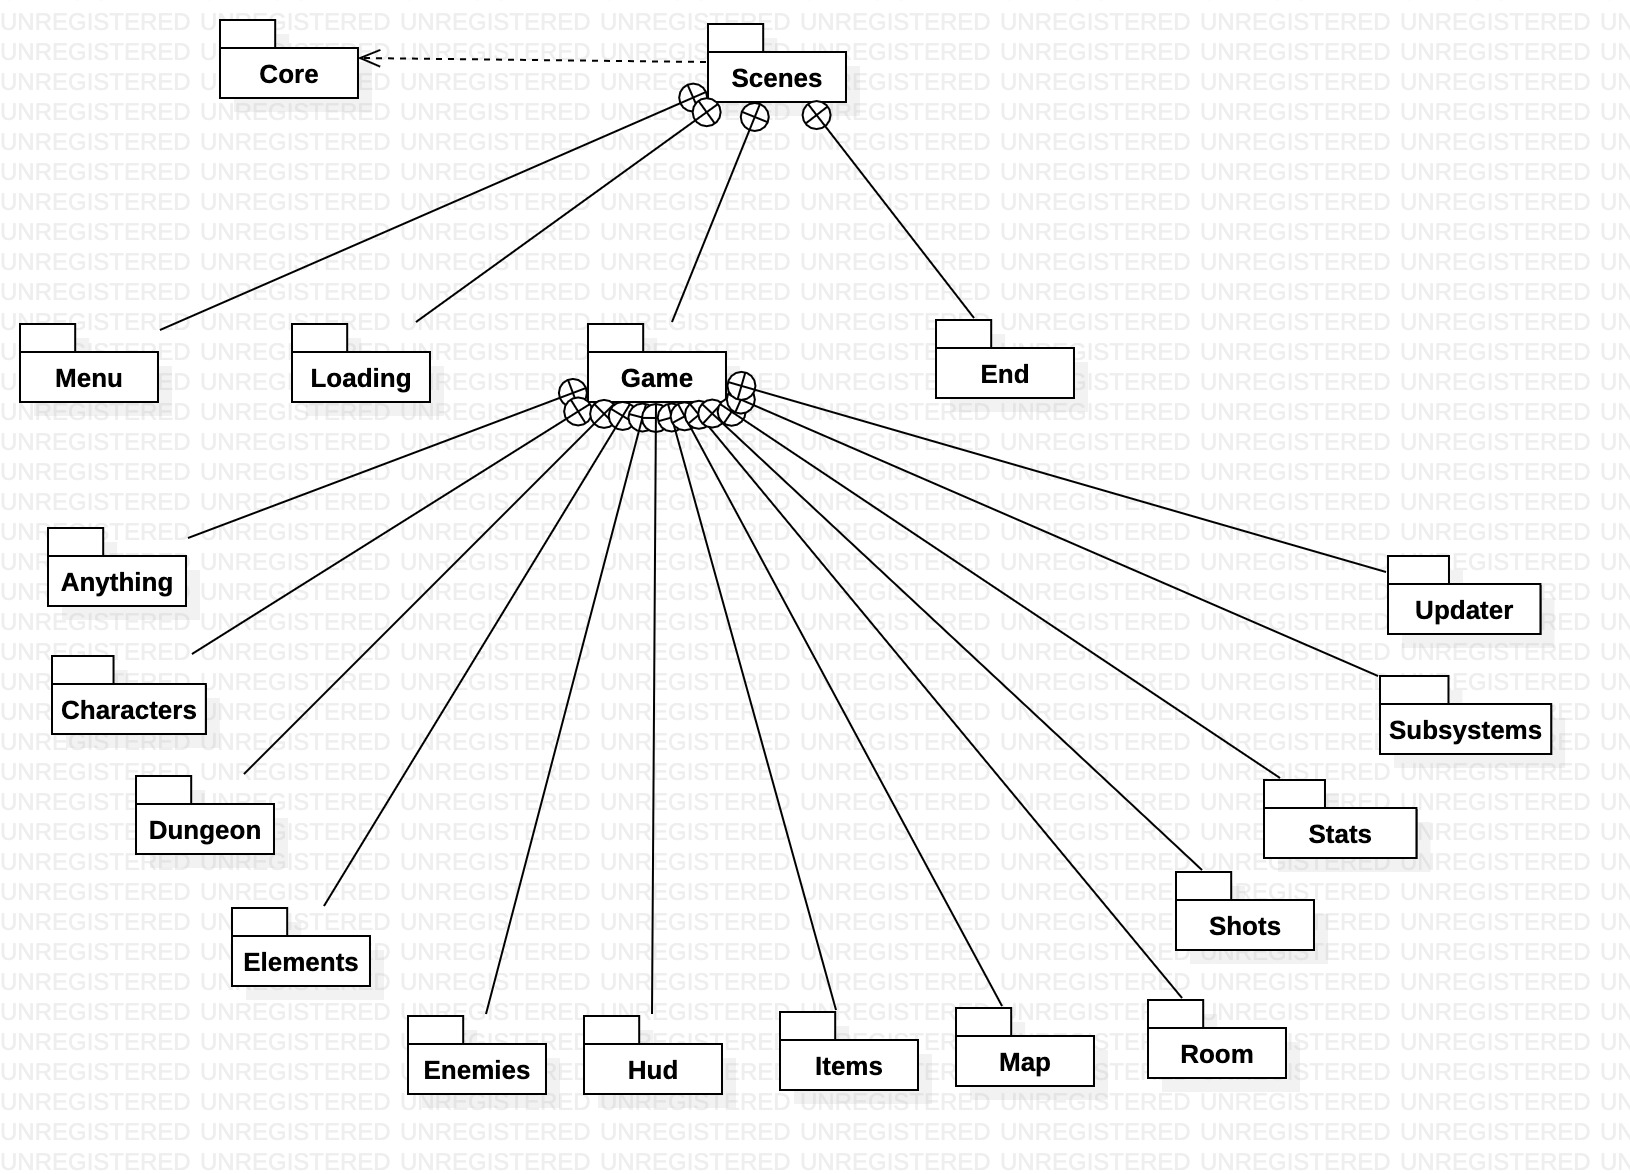
\includegraphics[scale=0.28]{package-diagram.jpg}
    \caption{\textit{Package Diagram del sistema(da modificare con versione pro di staruml)}} 
\end{figure}